\documentclass[12pt]{article}
\title{Assignment 3: CS 754, Advanced Image Processing}
\author{\textbf{Group Details:} \\
Vinit Awale (18D070067)\\ 
Piyush Bharambe (18D070019)
}
\date{}
\usepackage{amsmath}
\usepackage{amssymb}
\usepackage{hyperref}
\usepackage{ulem}
\usepackage{enumitem}
\usepackage{float}
\usepackage{graphicx}
\usepackage{subcaption}
\usepackage{bm}
\pagenumbering{gobble}

\usepackage[margin=0.5in]{geometry}
\begin{document}
\maketitle
\begin{center}
    \section*{Question 1}
\end{center}

\begin{itemize}
    \item Your task here is to implement the ISTA algorithm for the following three cases:
\begin{enumerate}
\item Consider the image from the homework folder. Add iid Gaussian noise of mean 0 and variance 3 (on a [0,255] scale) to it, using the `randn' function in MATLAB. Thus $\boldsymbol{y} = \boldsymbol{x} + \boldsymbol{\eta}$ where $\boldsymbol{\eta} \sim \mathcal{N}(0,3)$ \textcolor{blue}{(earlier the variance was mistakenly marked as 4)}. You should obtain $\boldsymbol{x}$ from $\boldsymbol{y}$ using the fact that patches from $\boldsymbol{x}$ have a sparse or near-sparse representation in the 2D-DCT basis. 
\item Divide the image shared in the homework folder into patches of size $8 \times 8$. Let $\boldsymbol{x_i}$ be the vectorized version of the $i^{th}$ patch. Consider the measurement $\boldsymbol{y_i} = \boldsymbol{\Phi x_i}$ where $\boldsymbol{\Phi}$ is a $32 \times 64$ matrix with entries drawn iid from $\mathcal{N}(0,1)$. Note that $\boldsymbol{x_i}$ has a near-sparse representation in the 2D-DCT basis $\boldsymbol{U}$ which is computed in MATLAB as `kron(dctmtx(8)',dctmtx(8)')'. In other words, $\boldsymbol{x_i} = \boldsymbol{U \theta_i}$ where $\boldsymbol{\theta_i}$ is a near-sparse vector. Your job is to reconstruct each $\boldsymbol{x_i}$ given $\boldsymbol{y_i}$ and $\boldsymbol{\Phi}$ using ISTA. Then you should reconstruct the image by averaging the overlapping patches. You should choose the $\alpha$ parameter in the ISTA algorithm judiciously. Choose $\lambda = 1$ (for a [0,255] image). Display the reconstructed image in your report. State the RMSE given as $\|X(:)-\hat{X}(:)\|_2/\|X(:)\|_2$ where $\hat{X}$ is the reconstructed image and $X$ is the true image. \textsf{[15 points]}
\end{enumerate}
\textbf{Answer:}
\begin{enumerate}
    \item The original and the noisy (Gaussian Noise of standard deviation 3) Barbara images are shown below.
    \begin{figure}[H]
        \centering
        \begin{minipage}{.45\textwidth}
            \centering
            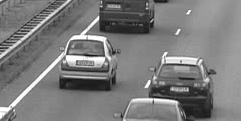
\includegraphics[width=\linewidth]{results/cars_3_orig_1.png}
            \caption*{Frame 1}
        \end{minipage}
        \begin{minipage}{.45\textwidth}
            \centering
            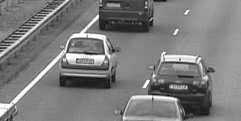
\includegraphics[width=\linewidth]{results/cars_3_orig_2.png}
            \caption*{Frame 2}
        \end{minipage}
    \end{figure}
\end{enumerate}
\end{itemize}
\end{document}
